\begin{figure}[H]
    \centering
    \begin{subfigure}{0.4\linewidth}
        \centering
        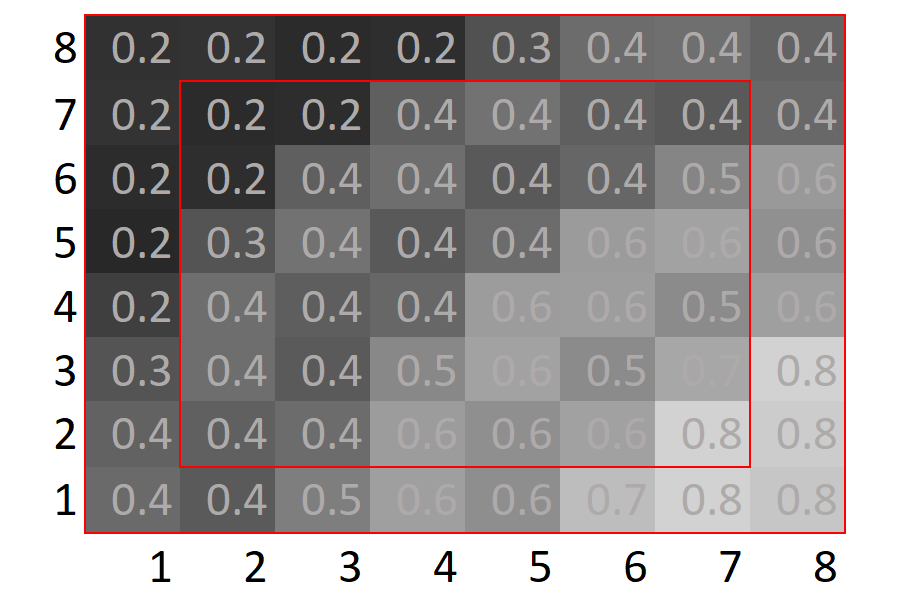
\includegraphics[width=0.8\linewidth]{image/boundary_condition/show_bounary.png}
    \end{subfigure}
    \begin{subfigure}{0.4\linewidth}
        \centering
        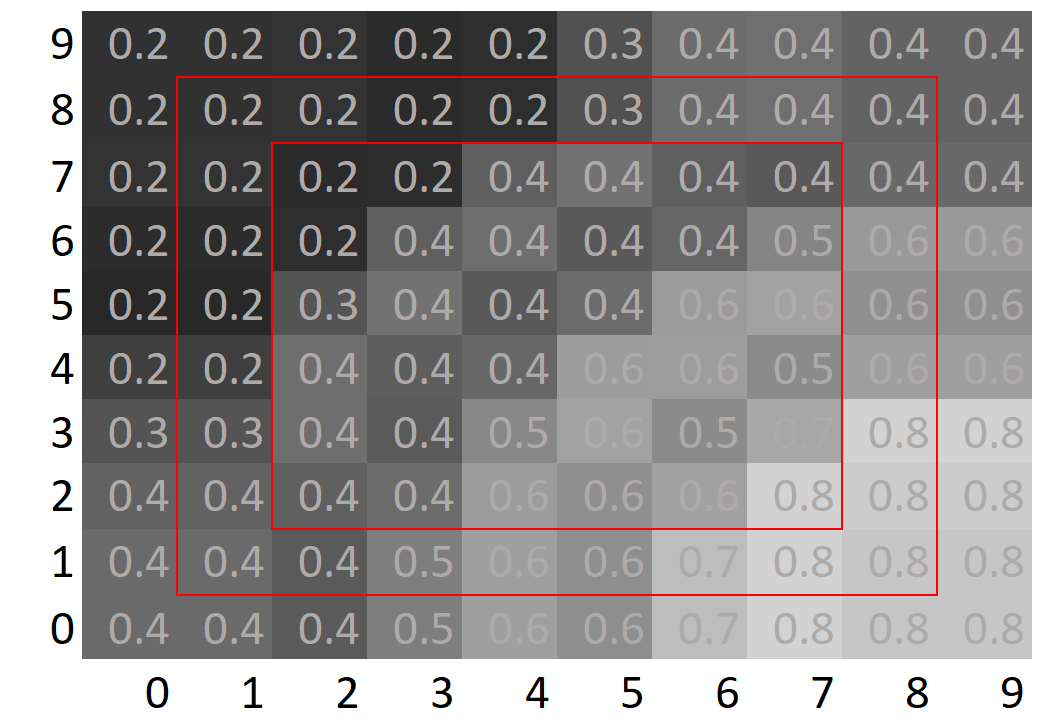
\includegraphics[width=0.8\linewidth]{image/boundary_condition/extend_edge_neuman.png}
    \end{subfigure}
    \label{figure:boundary_condition}
    \caption{ตัวอย่างภาพขอบเขตแบบนิวแมน}
\end{figure}